\documentclass[10pt,letterpaper]{article}
\usepackage[margin=1in,headheight=14pt]{geometry}
\usepackage[T1]{fontenc}
\usepackage{lmodern}
\usepackage{amsmath,amssymb,amsthm,mathtools}
\usepackage{microtype,booktabs,xcolor,fancyhdr,graphicx}
\definecolor{ink}{HTML}{19354A}
\usepackage[colorlinks=true,linkcolor=ink,urlcolor=ink,citecolor=ink]{hyperref}
\hypersetup{pdftitle={Exact probabilities of rainbow perfect matchings},pdfauthor={Akhil Ravuri}}
\graphicspath{{../results/figures/}{results/figures/}}
\newtheorem{proposition}{Proposition}
\newcommand{\E}{\mathbb E}
\newcommand{\Prob}{\mathbb P}
\pagestyle{fancy}\fancyhf{}
\fancyhead[L]{\small\textsc{Random edge colors}}
\fancyhead[R]{\small Akhil Ravuri}\fancyfoot[C]{\thepage}
\renewcommand{\headrulewidth}{0.3pt}
\setlength{\parskip}{0.2em}\setlength{\emergencystretch}{1em}
\title{\vspace{-1.5em}\LARGE\bfseries Exact probabilities of\\rainbow perfect matchings}
\author{Akhil Ravuri}\date{}
\begin{document}
\maketitle\vspace{-1.5em}
\begin{abstract}
We convert exhaustive edge-partition counts into exact probabilities under
independent uniform edge colors. Matching intersections give first- and
second-moment bounds, while the largest avoiding partitions determine a
large-palette limit. Six fixed hosts illustrate the formulas. This note
typesets the repository's existing counting arguments and finite results;
no novelty is claimed.
\end{abstract}

\section{Model and partition weights}
Let $G$ be a finite graph with $m\ge1$ edges and at least one perfect matching.
Every edge receives an independent uniform color from $\{1,\ldots,q\}$,
where $q\ge1$ is an integer. Colors are \emph{available}, not necessarily all
used, and colorings need not be proper. A matching is rainbow when its edges
have pairwise distinct colors.

Let $a_k$ count partitions of the fixed edge set into $k$ nonempty color
classes that avoid every rainbow perfect matching. Color names are ignored;
graph symmetries are not identified. Write
\[
 (q)_k=q(q-1)\cdots(q-k+1),\qquad (q)_0=1,
\]
with $(q)_k=0$ for $k>q$.
\begin{proposition}\label{prop:weights}
The probability of at least one rainbow perfect matching is
\[
 \Prob(X>0)=1-q^{-m}\sum_k a_k(q)_k,
\]
where $X$ is the number of rainbow perfect matchings.
\end{proposition}
\begin{proof}
Each named coloring determines a unique partition into equal-color classes.
A fixed partition with $k$ blocks receives distinct palette labels in exactly
$(q)_k$ ways. These classes of assignments are disjoint, and every one of the
$q^m$ assignments has probability $q^{-m}$. Summing the avoiding assignments
and taking the complement proves the identity.
\end{proof}
Uniformly sampling partitions would give a different distribution: partitions
with different numbers of blocks have different numbers of labelings.

\section{Matching overlap and moment bounds}
Suppose each perfect matching has $n$ edges and there are $N$ perfect matchings.
For each matching $M$, let $I_M$ indicate that it is rainbow, so
$X=\sum_M I_M$. A single matching has rainbow probability
\[
 p=\frac{(q)_n}{q^n},\qquad \E[X]=Np.
\]
For distinct matchings $M,M'$ sharing $s$ edges, the joint probability is zero
if $q<n$. If $q\ge n$, it is
\begin{equation}\label{eq:joint}
 \Prob(I_M=I_{M'}=1)=\frac{(q)_n(q-s)_{n-s}}{q^{2n-s}}.
\end{equation}
Indeed, conditional on $M$ being rainbow, its $s$ shared edges have distinct
colors. The other $n-s$ edges of $M'$ must avoid those colors and have mutually
distinct colors. This gives $(q-s)_{n-s}$ choices among $q^{n-s}$ assignments.
They may reuse colors from the unshared edges of $M$. Thus
\[
 \E[X^2]=Np+2\sum_{\{M,M'\}}\Prob(I_M=I_{M'}=1),
\]
where the sum is over unordered distinct pairs. Shared-edge counts zero and
one give pairwise independence of these indicators; the whole family need
not be mutually independent.

\begin{proposition}\label{prop:bounds}
If $\E[X^2]>0$, then
\[
 \frac{\E[X]^2}{\E[X^2]}\le \Prob(X>0)\le\min\{1,\E[X]\}.
\]
If $\E[X^2]=0$, the probability and both bounds are zero.
\end{proposition}
\begin{proof}
The upper bound follows from $X\ge\mathbf1_{\{X>0\}}$. For the lower bound,
write $u=\Prob(X>0)>0$. Nonnegative conditional variance gives
\[
 \E[X^2]=u\E[X^2\mid X>0]
 \ge u\E[X\mid X>0]^2=\frac{\E[X]^2}{u}.
\]
Rearrange. If the second moment is zero, the nonnegative integer $X$ is zero
almost surely, so no division is needed.
\end{proof}

\section{Exact finite comparison}
The saved partition histograms give the following values. The crossing column
is the first positive integer palette size whose probability is at least
$1/2$, checked against every smaller positive integer. Percentages are rounded
to two decimal places; calculations use exact fractions.
\begin{center}
\begin{tabular}{lrrrrr}
\toprule
Host & Edges & Matchings & First $q$ & $q=4$ & $q=8$\\
\midrule
$C_4$ & 4 & 2 & 2 & $93.75\%$ & $98.44\%$\\
$C_6$ & 6 & 2 & 4 & $60.94\%$ & $88.18\%$\\
$C_8$ & 8 & 2 & 7 & $17.87\%$ & $65.21\%$\\
$C_4\sqcup C_4$ & 8 & 4 & 5 & $31.49\%$ & $84.31\%$\\
$K_{3,3}$ & 9 & 6 & 3 & $93.64\%$ & $99.76\%$\\
Cube $Q_3$ & 12 & 9 & 4 & $56.80\%$ & $98.15\%$\\
\bottomrule
\end{tabular}
\end{center}
For example, on the cube with $q=4$,
\[
 \E[X]=\frac{27}{32},\qquad \E[X^2]=\frac{99}{64},\qquad
 \frac{81}{176}\le\Prob(X>0)=\frac{4653}{8192}\le\frac{27}{32}.
\]
Expectation differs from existence probability because a coloring can contain
several rainbow matchings. An eight-color palette also does not force a
rainbow cube matching: the sampled assignment may use fewer than eight colors.
This is consistent with the extremal maximum of seven colors actually used.

\begin{figure}[htbp]
\centering
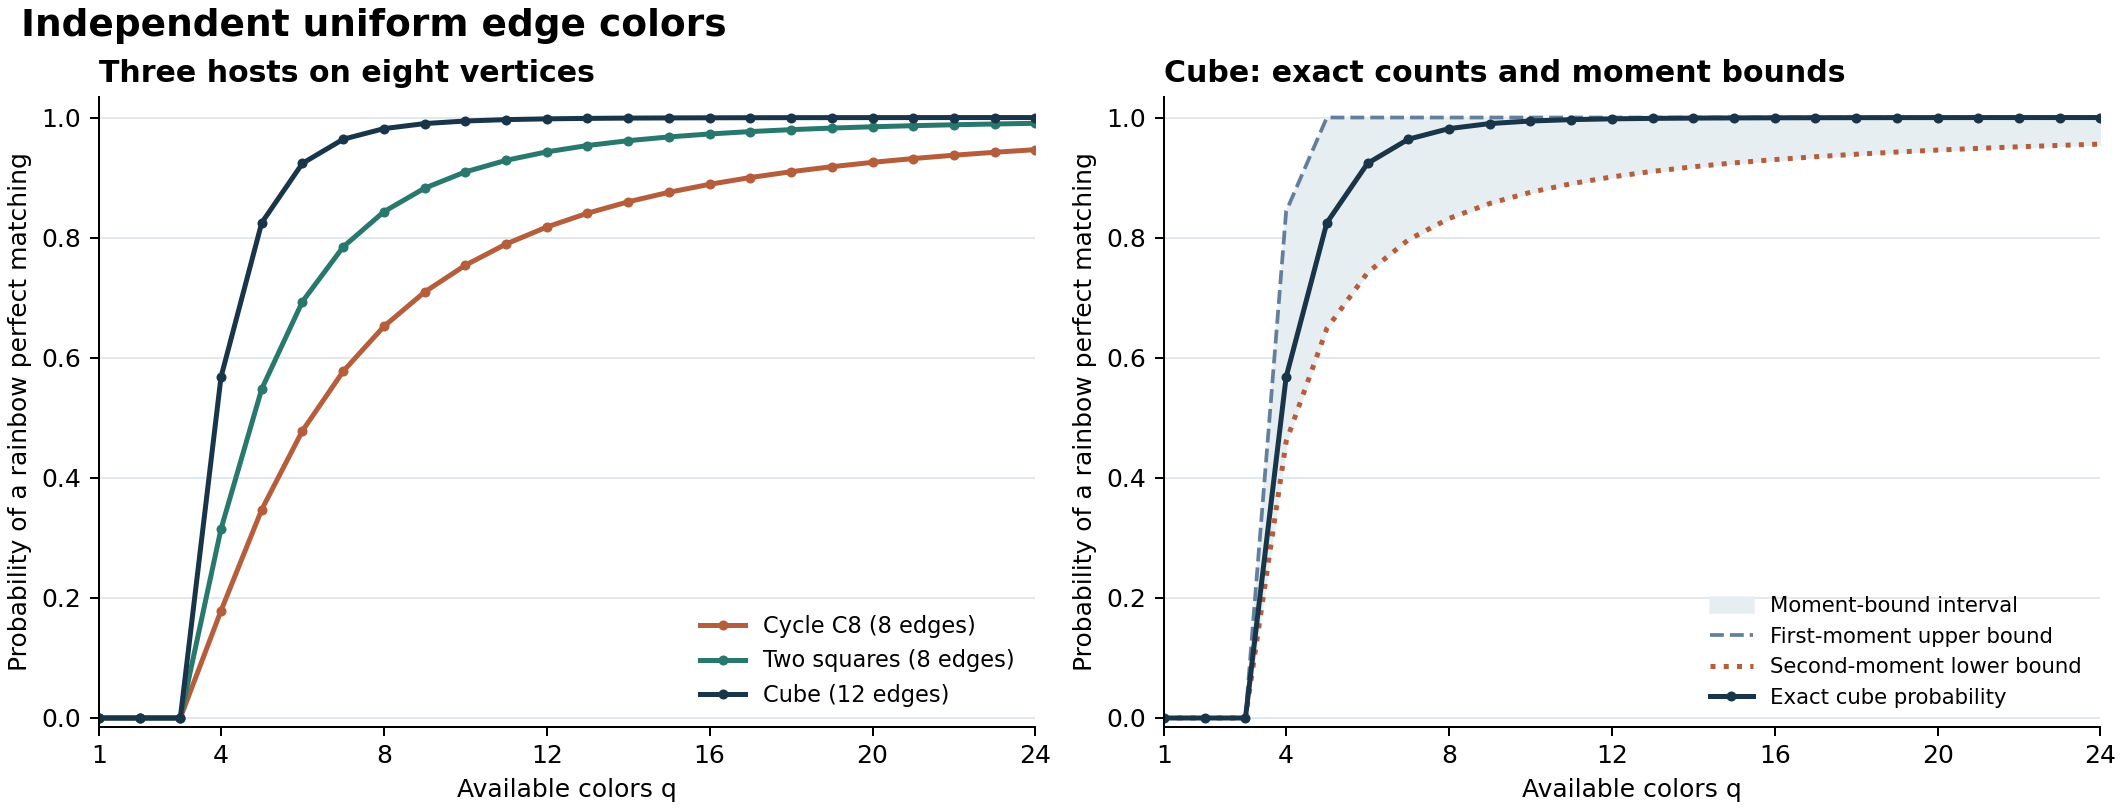
\includegraphics[width=\linewidth]{random_rainbow.png}
\caption{Exact probabilities on three eight-vertex hosts and analytic cube
bounds. Points represent integer palette sizes; lines guide the eye. Shading
is the interval between moment bounds, not statistical uncertainty.}
\end{figure}

\section{Checks and the large-palette tail}
An even cycle $C_{2n}$, $n\ge2$, has two alternating perfect matchings on
disjoint edge sets. Their rainbow events are independent, so
\[
 \Prob(X>0)=1-\left(1-\frac{(q)_n}{q^n}\right)^2.
\]
This supplies an oracle separate from histogram weighting.

\begin{proposition}
Assume an avoiding coloring exists and set $A=\max\{k:a_k>0\}$. Then, as
$q$ tends to infinity through the positive integers,
\[
 q^{m-A}\Prob(X=0)\longrightarrow a_A.
\]
\end{proposition}
\begin{proof}
Every $(q)_k$ is monic of degree $k$. The sum in
Proposition~\ref{prop:weights} therefore has leading term $a_Aq^A$.
Multiply the avoidance probability by $q^{m-A}$ and take the limit.
\end{proof}
For the cube, the incidence proof gives $A=7$ and the exhaustive classification
gives $a_7=174$. Consequently $q^5\Prob(X=0)\to174$. The saved scaled values
at $q=32$ and $1024$ are approximately $361.18$ and $180.72$; the limit need
not be a good approximation for small palettes. The polynomial argument
proves the limit; the numerical examples only illustrate it.

\subsection*{Reproduction and scope}
The implementation is \path{src/rainbow_probability.py}. From the repository
root, run
\begin{quote}\small\ttfamily
python -m experiments.random\_rainbow\par
python -m unittest discover -s tests -v
\end{quote}
The reference file \path{results/data/random_rainbow.json} contains 144
main-grid rows: six hosts and $q=1,\ldots,24$, plus five larger cube palettes.
Checks use direct named-color enumeration on $C_4$, $C_6$, and two disjoint
squares, the independent cycle formula, and four-position overlap-event
oracles. All main-grid bounds are checked exactly. No sampling or numerical
tolerance establishes these results. The figure alone uses floating-point
conversion. The cube's coefficient depends on its finite classification;
no new graph-family threshold or literature novelty follows.

\subsection*{Companion records}
Definitions and proofs are also readable in
\href{https://github.com/Akhil-rav/discrete-math-lab/blob/main/notes/random_rainbow.md}{the counting note}.
The repository's
\href{https://github.com/Akhil-rav/discrete-math-lab/blob/main/results/random_rainbow_verification.md}{verification record}
states the original review and execution scope. The
\href{https://github.com/Akhil-rav/discrete-math-lab/blob/main/results/cube_classification.md}{cube classification}
supplies the 174-partition count.
\end{document}
